\documentclass[12pt]{beamer}

\usetheme{metropolis}
\usepackage{amsmath, amssymb, graphicx, booktabs}

\title{AMS 572 Project (Group 6)}
\author{Benjamin Minkin, Marcus Minutello, Jacob White \\ AMS 572}
\date{Due: December 5, 2025 at 10:00am}

\begin{document}
	\frame{\titlepage}
	
	\begin{frame}{What is our project about?}
		Bitcoin has evolved from a niche digital token into a globally traded financial asset:
		
		\begin{itemize}
			\item Held by hedge funds, Fortune 500 companies, and national banks.
			\item Increasing adoption as legal tender and payment medium (e.g., in El Salvador).
			\item Growth of broader cryptocurrency ecosystem.
		\end{itemize}
		
		Two cryptocurrency types:
		\begin{itemize}
			\item \textbf{Native coins} – technological improvements.
			\item \textbf{Memecoins} – speculative, hype-driven assets.
		\end{itemize}
	\end{frame}
	
	\begin{frame}{Questions of Interest}
		\textbf{Question 1}: Does Bitcoin’s price movement follow that of the S\&P 500?
		
		\textbf{Question 2}: Do memecoins follow Bitcoin’s price changes more than native coins?
		
		\bigskip
		
		Understanding these questions informs:
		\begin{itemize}
			\item Bitcoin’s diversification value,
			\item The speculative nature of memecoins,
			\item Differences between crypto assets driven by "hype" and those driven by sought-after utility. 
		\end{itemize}
	\end{frame}
	\begin{frame}{Data Description}
		Data collected from Yahoo Finance using \texttt{quantmod} in \texttt{R}:
		
		\begin{itemize}
			\item Date range: Nov 1, 2023 – Nov 18, 2025.
			\item Log-returns computed via $ r_t = \log(P_t/P_{t-1}) $.
			\item Coins categorized as native vs.\ memecoin.
		\end{itemize}
		
		\begin{figure}
			\centering
			
\includegraphics[width=0.8\linewidth]{q1_1_growth.png}
		\end{figure}
	\end{frame}
	
	\begin{frame}{Background on Financial Time Series}
		A financial time series records prices or returns over time.
		
		\begin{itemize}
			\item Log-returns preferred for additivity and approximate normality.
			\item Efficient market hypothesis suggests log returns follow a random walk.
		\end{itemize}
		
		\begin{figure}
			\centering
			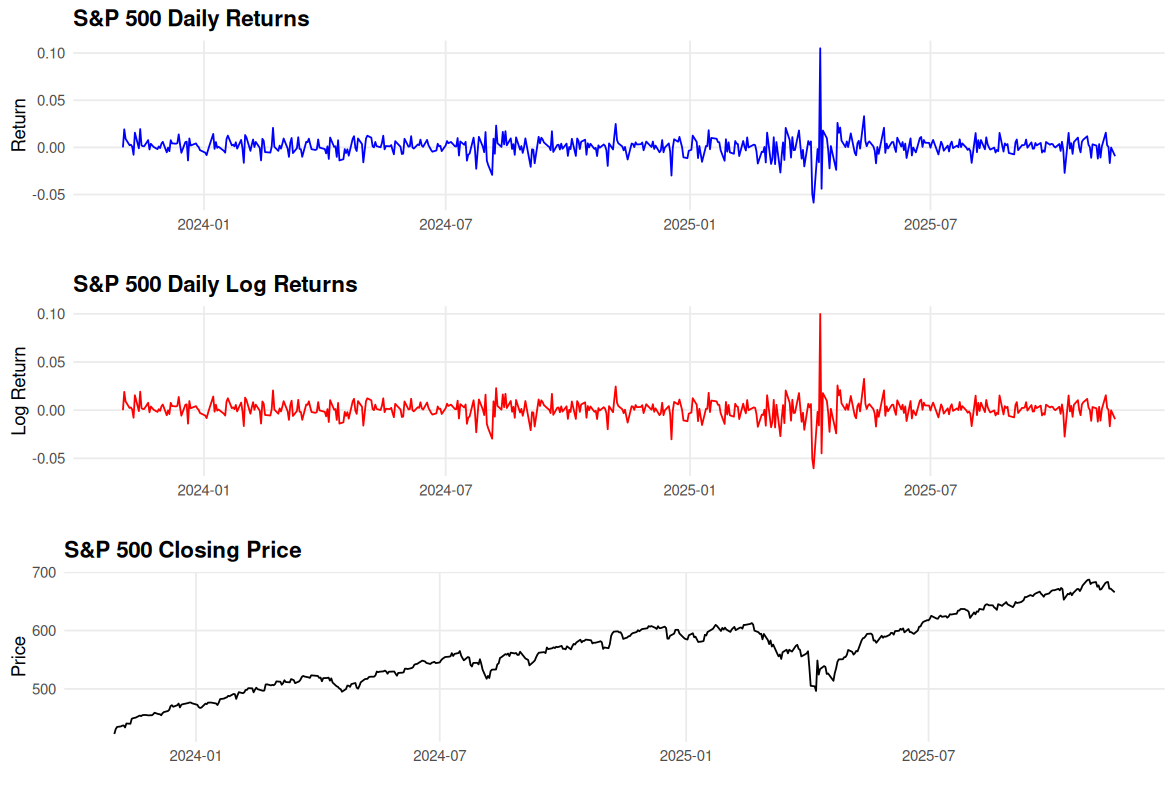
\includegraphics[width=0.6\linewidth]{572_SP500_ret.png}
			\caption{Example of SPY daily log returns.}
		\end{figure}
	\end{frame}
	
	\begin{frame}{Correlation Between Time Series}
		Pearson correlation coefficient:
		
		$$\hat{\rho} = \frac{\sum (x_t - \bar{x})(y_t - \bar{y})}{\sqrt{\sum(x_t-\bar{x})^2}\sqrt{\sum(y_t-\bar{y})^2}}$$
		
		Used to test:
		$$
		H_0: \rho = 0.
		$$
		
	\end{frame}
	
	\begin{frame}{BTC vs. Spy Log Returns}
		\begin{figure}
			\centering
			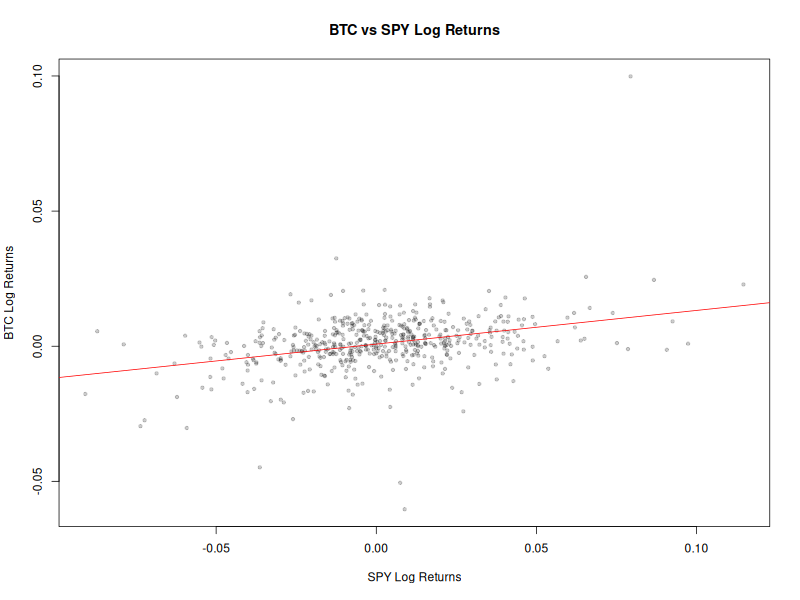
\includegraphics[width=0.75\linewidth]{diag_linearity.png}
			\caption{BTC vs.\ SPY log-return scatterplot.}
		\end{figure}
	\end{frame}
	\begin{frame}{Multiple Linear Regression with Interaction}
		Model:
		\begin{align*}
		&\mathrm{Return}_{i,t} =
		\beta_0 + \beta_1 \mathrm{BTC}_t +
		\beta_2 \mathrm{Memecoin}_i  \\
		&+ \beta_3 (\mathrm{BTC}_t \cdot \mathrm{Memecoin}_i)
		+ \varepsilon_{i,t}.
		\end{align*}
		
		Interpretation:
		\begin{itemize}
			\item \(\beta_1\): BTC sensitivity of native coins.
			\item \(\beta_3\): \textbf{Additional} sensitivity of memecoins.
		\end{itemize}
		
		
	\end{frame}
	
	\begin{frame}{Multiple Linear Regression with Interaction}
		\begin{figure}
			\centering
			
\includegraphics[width=0.75\linewidth]{q2_3_native_grid_scatter.png}
			\caption{Native coin returns vs.\ BTC.}
		\end{figure}
	\end{frame}
	
	\begin{frame}{Memecoin Scatterplots}
		\begin{figure}
			\centering
			
\includegraphics[width=0.8\linewidth]{q2_4_meme_grid_scatter.png}
			\caption{Memecoin returns vs.\ BTC.}
		\end{figure}
		
		 Steeper slopes, but much greater volatility. 
	\end{frame}
	
	
	\begin{frame}{Distribution and Autocorrelation Diagnostics}
		\begin{figure}
			\centering
			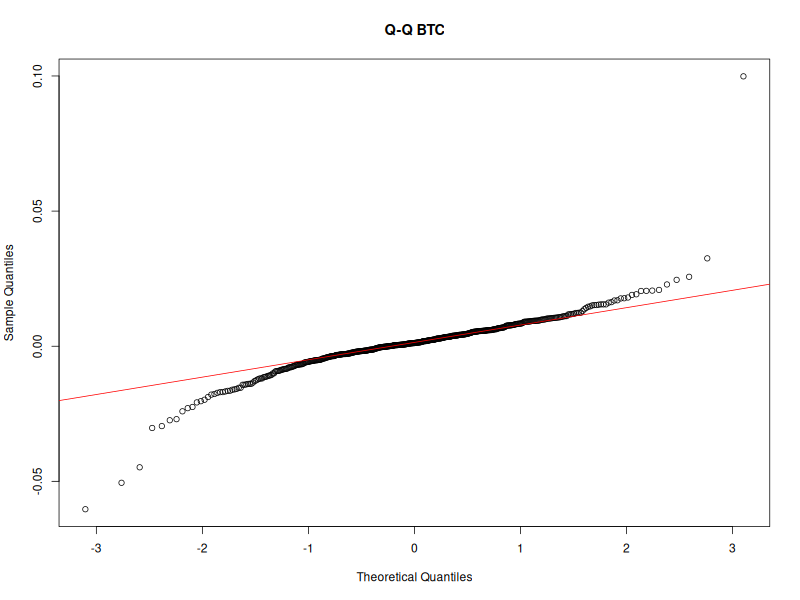
\includegraphics[width=0.45\linewidth]{diag_qq_btc.png}
			\hspace{0.4cm}
			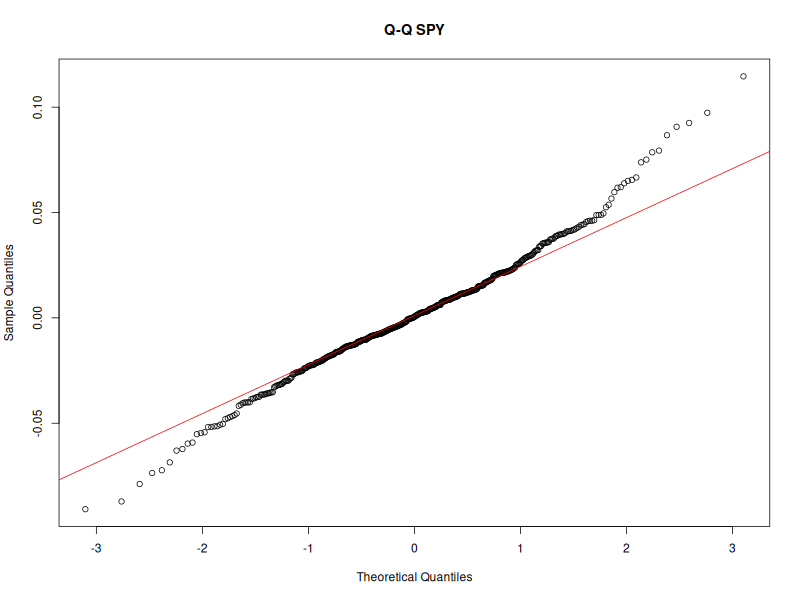
\includegraphics[width=0.45\linewidth]{diag_qq_spy.png}
			\caption{Q–Q plots for BTC and SPY.}
		\end{figure}
		
		
	\end{frame}
	\begin{frame}{ACF of BTC log-returns}
		\begin{figure}
			\centering
			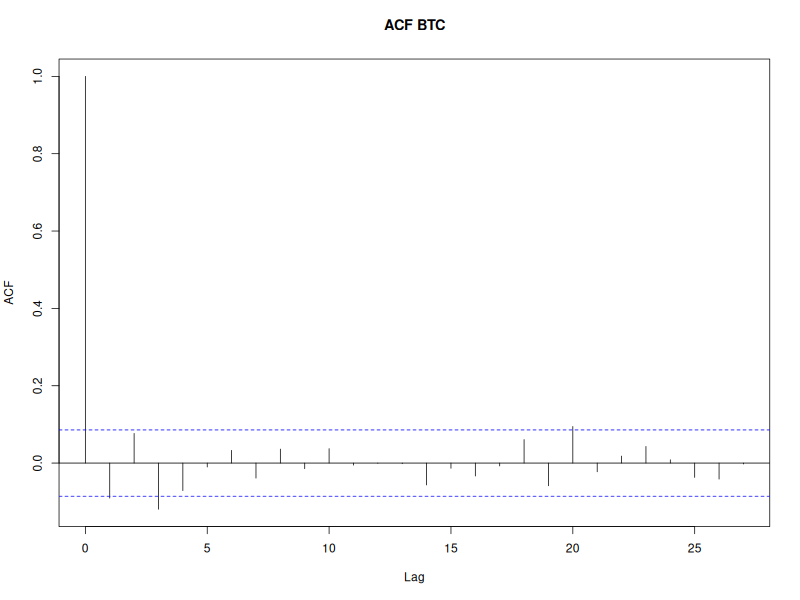
\includegraphics[width=0.65\linewidth]{diag_acf_btc.png}
			\caption{ACF of BTC log-returns.}
		\end{figure}
	\end{frame}
	
	\begin{frame}{Regression Diagnostics}
		\begin{figure}
			\centering
			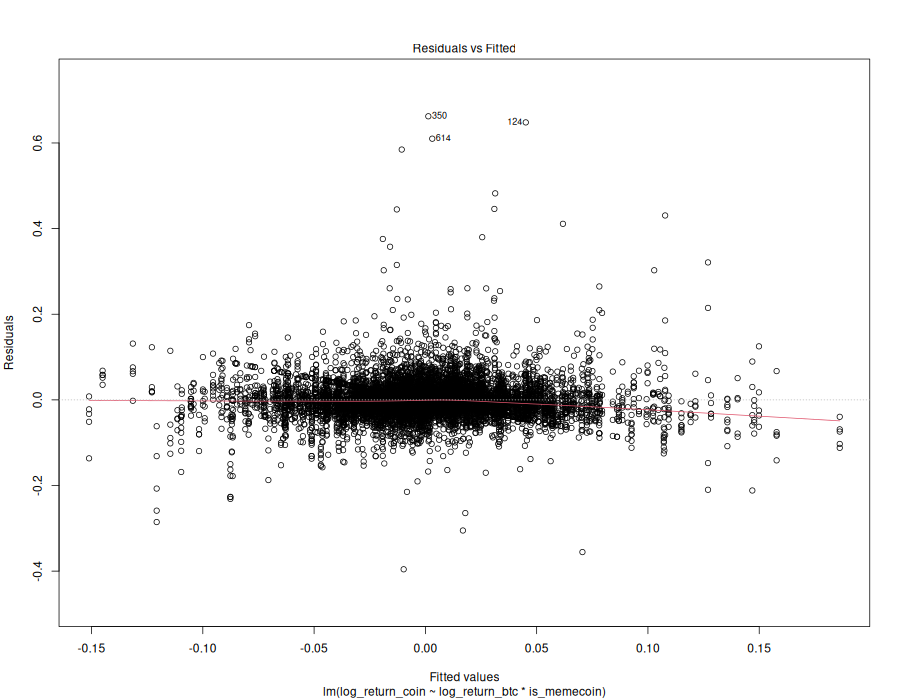
\includegraphics[width=0.45\linewidth]{q2_diag_residuals_vs_fitted.png}
			\hspace{0.4cm}
			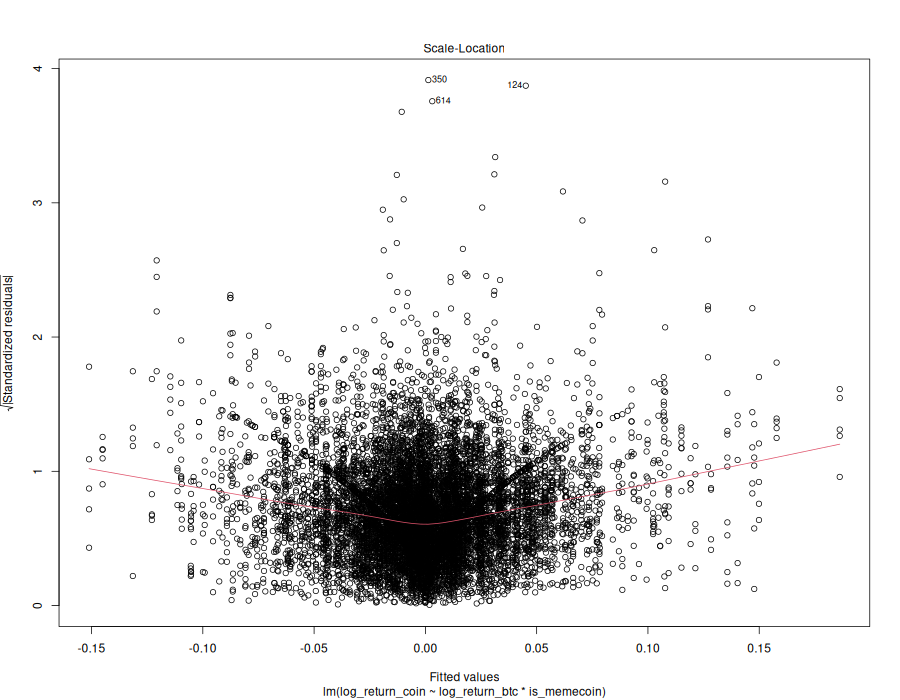
\includegraphics[width=0.45\linewidth]{q2_diag_scale_location.png}
			\caption{\textbf{Left}: Residuals vs. Fitted, \quad \textbf{Right}: Scale-Location.}
		\end{figure}
	\end{frame}
	
	
	\begin{frame}{Question 1 Results}
		\[
		\hat{\rho} = 0.3499 \quad p = 2.07 \times 10^{-15}.
		\]
		
		\textbf{Conclusion:}  
		Bitcoin's returns significantly correlate with S\&P 500 returns.
		
		Missing data effects:
		\begin{itemize}
			\item MCAR: \(\hat{\rho}_{MCAR}=0.3637\)
			\item MNAR: \(\hat{\rho}_{MNAR}=0.3037\)
		\end{itemize}
		
		Correlation remained statistically significant in both cases.
	\end{frame}
	
	\begin{frame}{Question 2 Results}
		
		$$\beta_3 = 0.4627,\quad p = 4.96 \times 10^{-10}.$$
		
		
		\textbf{Conclusion:}
		\begin{itemize}
			\item Memecoins exhibit significantly stronger BTC sensitivity than native coins.
		\end{itemize}
		
		Missing data effects:
		\begin{itemize}
			\item MCAR: $\beta_{3,MCAR} = 0.4515$
			\item MNAR: $\beta_{3,MNAR} = 0.2319$
		\end{itemize}
	\end{frame}
	
	\begin{frame}{Summary of Findings}
		\textbf{1. Bitcoin shows moderate correlation with the S\&P 500.}
		
		\textbf{2. Memecoins exhibit greater BTC sensitivity than native coins.}
		
		Implications:
		\begin{itemize}
			\item Bitcoin behaves increasingly like a traditional asset.
			\item Memecoins are much more sensitive to price changes in BTC than native coins. 
			\item Native coins behave more like utility-driven blockchain assets.
		\end{itemize}
	\end{frame}
	
	\begin{frame}{Limitations \& Future Work}
		Limitations:
		\begin{itemize}
			\item Violations of time-series assumptions.
			\item Two-year sample window.
			\item Selection bias. 
		\end{itemize}
		
		Future work:
		\begin{itemize}
			\item Explore longer time horizons (this study was limited to about 2 years).
			\item Consider more crypto assets. 
			\item Develop more detailed cryptocurrency categorization (i.e., consider properties of each cryptocurrency's implementation, and categorize based off these properties).
		\end{itemize}
	\end{frame}
	
	%----------------------------------------------------------
	\begin{frame}{}
		\centering \Large Thank you!
	\end{frame}
	%----------------------------------------------------------
	
\end{document}
